% Ideia geral

As \emph{Redes Neurais Artificiais} (RNAs) são modelos computacionais inspirados na capacidade de processamento de informações do cérebro humano \cite{ref:rojas}. De acordo com esta ideia, as RNAs possuem unidades de processamento simples, denominadas \emph{neurônios artificiais}, dispostos em camadas interconectadas por ligações associadas a coeficientes numéricos, chamados \emph{pesos} \cite{ref:faceli}. As RNAs são capazes de aprenderem padrões complexos a partir dos dados e prever resultados para exemplos não conhecidos, o que demonstra a sua capacidade de generalização \cite{ref:haykin}.

% Neurônio Artificial

O neurônio artificial é a unidade fundamental na construção de RNAs, tendo sido inspirado no seu análogo biológico. Segundo Rosenblatt, existe um conjunto de $m$ entradas, equivalentes aos dendritos de um neurônio biológico, por onde os sinais são introduzidos \cite{ref:rosenblatt}. Associa-se um peso a cada entrada, representando a relevância referente a uma conexão sináptica. Há também o peso $w_0$, um termo de polarização criado com a intenção de estabelecer um limiar de ativação para cada neurônio. Este peso corresponde à entrada \emph{bias}, cujo valor é sempre unitário. Pode-se então definir um vetor de entradas $X = [+1, x_1, x_2, \ldots, x_m]$ e um vetor de pesos $W = [w_0, w_1, \ldots, w_m$]. As entradas e pesos são combinados por meio de uma função $\phi: \mathbbm{R}^{m+1} \rightarrow \mathbbm{R}$, que é geralmente a soma ponderada das entradas e pesos, conforme Equação \ref{eq:somaPonderada}. Este modelo de neurônio encontra-se ilustrado na Figura \ref{img:neuronioArtificial} \cite{ref:patrick-tcc}.

\begin{equation}
\phi(X,W) = \sum_{i =0}^m x_i \cdot w_i. \label{eq:somaPonderada}
\end{equation}

\begin{figure}[!ht]
	\centering
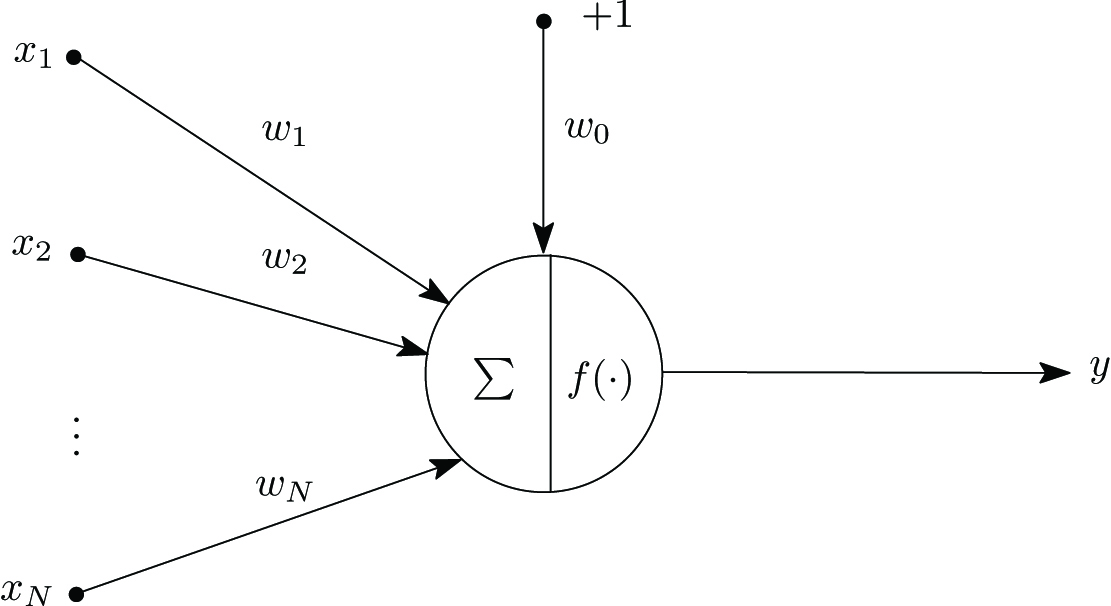
\includegraphics[width=0.6\textwidth]{./img/neuron}
\caption{Neurônio artificial: a combinação linear das entradas \emph{x} ponderadas pelos pesos \emph{w} é transformada pela função de ativação \emph{f} na saída \emph{y}.}
\label{img:neuronioArtificial}
\end{figure}

% Funções de ativação

A função $f$ é chamada de \emph{função de ativação} e fornece a resposta de um neurônio para uma dada entrada. Esta função precisa ser monotônica e contínua, podendo comumente ser as funções identidade, sigmóide, tangente hiperbólica, ou a retificada linear (ReLU) \cite{ref:JAI-2017}. Estas funções encontram-se representadas na Figura \ref{img:funcs_ativacao}.

\begin{figure}[!ht]
	\centering
	\subfloat[Função identidade. \label{img:func_id}]{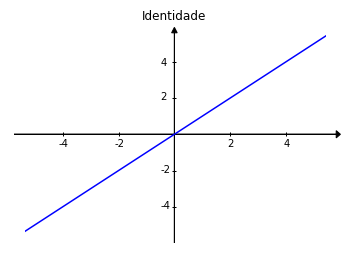
\includegraphics[width=0.4\linewidth]{./img/id}}
	\subfloat[Função sigmóide.\label{img:func_sigmoide}]{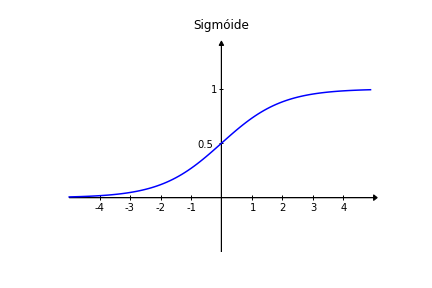
\includegraphics[width=0.4\linewidth]{./img/sigmoide}}\\
	\subfloat[Função tangente hiperbólica. \label{img:func_tanh}]{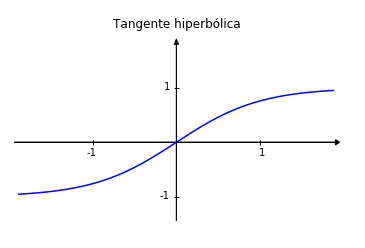
\includegraphics[width=0.4\linewidth]{./img/tanh}}
	\subfloat[Função retificada linear.\label{img:func_relu}]{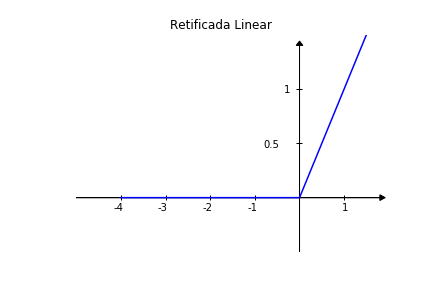
\includegraphics[width=0.4\linewidth]{./img/relu}}
	\caption{Exemplos de diferentes funções de ativação.}
	\label{img:funcs_ativacao}																																														
\end{figure}

% Camadas ocultas

Neurônios artificiais individuais têm uma capacidade computacional limitada, independentemente da função de ativação escolhida, pois resolvem apenas problemas linearmente separáveis. No entanto, um conjunto de neurônios artificiais conectados na forma de uma rede -- \emph{rede neural artificial} -- adquirem a capacidade de resolver problemas de elevada complexidade \cite{ref:teresa}. A alternativa mais utilizada para resolver estes problemas é distribuir os neurônios em uma ou mais camadas conhecidas como  camadas ocultas \cite{ref:faceli}. Segundo Cybenko, uma rede com uma camada oculta pode implementar qualquer função contínua e uma rede com duas camadas ocultas permite a aproximação de qualquer função \cite{ref:cybenko}.

% Multilayer Perceptron

As RNAs do tipo Perceptron Multicamadas (MLP, do inglês \emph{Multilayer Perceptron}) apresentam uma camada de entrada, uma ou mais camadas ocultas e uma camada de saída. Uma das principais características de uma rede MLP é o seu alto grau de conectividade entre os neurônios, cuja intensidade está associada aos pesos da rede.

Cada neurônio em uma rede MLP atua ponderando as entradas recebidas dos neurônios de uma camada anterior a ele conectados, produzindo como saída um valor, resultante de sua função de ativação, que é propagado às camadas seguintes da rede neural. Conforme exemplificado na Figura \ref{img:rede-mlp}, a combinação das atuações individuais desempenhadas por cada neurônio da rede que define a atuação associada à RNA como um todo \cite{ref:teresa,ref:faceli,ref:haykin}.


\begin{figure}[!ht]
	\centering
	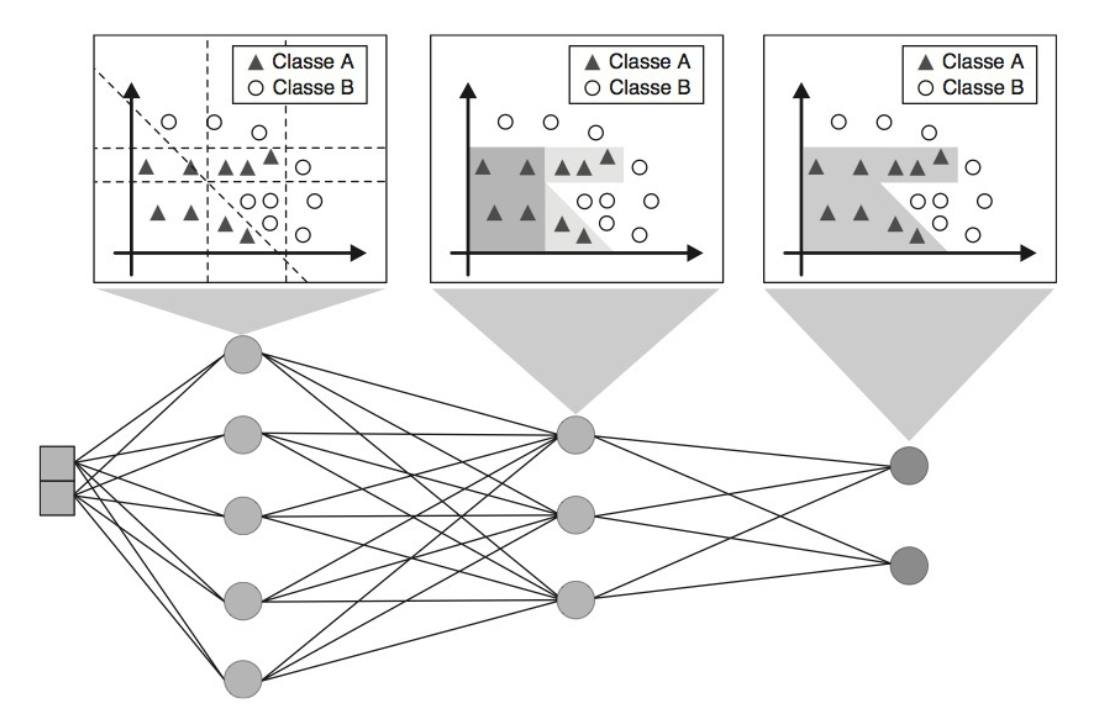
\includegraphics[width=1\textwidth]{./img/rede-mlp}
	\caption{Papel desempenhado pelos neurônios das diferentes camadas de uma rede MLP. Fonte: \cite{ref:faceli}.}
	\label{img:rede-mlp}
\end{figure}

% Aprendizado

Uma importante característica das RNAs é a sua capacidade de aprender por meio de exemplos. O processo de \emph{aprendizado} de uma rede neural consiste em sucessivos ajustes de pesos associados aos seus neurônios, de modo a aprimorar seu desempenho de acordo com um critério pré-estabelecido. Tais ajustes são realizados por algoritmos de treinamento formados por um conjunto de regras bem definidas que especificam quando e como deve ser alterado o valor de cada peso. Diversos algoritmos de aprendizado foram propostos, dentre os quais se destacam aqueles que seguem o paradigma de \emph{aprendizado supervisionado} \cite{ref:faceli,ref:patrick-tcc}.

% Paradigmas de aprendizado

O aprendizado supervisionado ajusta os pesos aplicando um conjunto de exemplos de treinamento rotulados. Cada exemplo consiste em um sinal de entrada associado à sua resposta alvo desejada. A cada padrão de entrada submetido à rede, compara-se a resposta desejada com a resposta calculada, ajustando-se os pesos das conexões para minimizar o erro \cite{ref:haykin}.

% Backpropagation

O algoritmo mais utilizado para o treinamento de redes MLP é o algoritmo \emph{backpropagation}, também chamado de retropropagação do erro ou ainda regra delta generalizada. Este algoritmo respeita o aprendizado supervisionado em que os pesos são modificados e ajustados para reduzir a distância entre a resposta desejada e a resposta produzida pela rede \cite{ref:haykin}. O treinamento é constituído da iteração de duas fases, uma fase para frente (\emph{forward}) e uma fase para trás (\emph{backwards}) \cite{ref:faceli}. A fase \emph{forward}, que compreende o fluxo da informação a partir da entrada até a saída da rede, é utilizada para produzir uma saída para um dado sinal de entrada. A fase \emph{backwards}, com fluxo da informação da saída da rede em direção à entrada, utiliza a diferença entre as saídas desejada e produzida para atualizar os pesos das conexões entre os neurônios e assim minimizar o erro \cite{ref:teresa}. Os ciclos de apresentação dos dados de treinamento e eventuais ajustes de pesos no \emph{backpropagation} são iterados até que seja atingido um critério de parada como, por exemplo, um número máximo de ciclos ou uma taxa máxima de erro \cite{ref:faceli}.


% Aplicações

As RNAs são modelos computacionais com ampla aplicação na resolução de problemas de previsão. Algumas aplicações utilizam RNAs para predição de condições climáticas, como em \cite{ref:apl-clima1} e \cite{ref:apl-clima2}, em que se deseja prever precipitações de chuva de determinados locais. Diversas outras aplicações de RNAs dizem respeito à classificação de padrões. Dentre as aplicações na área de classificação financeira, uma das mais bem sucedidas é a análise de crédito \cite{ref:teresa}. Além disso, as RNAs também são muito utilizadas para diagnósticos médicos, como em \cite{ref:apl-diagnostico1} e \cite{ref:apl-diagnostico2}. Outras aplicações tratam de reconhecimento de caracteres \cite{ref:apl-caracteres}, robótica \cite{ref:apl-robotica}, jogos \cite{ref:apl-jogos}, comunicação \cite{ref:meu-artigo}, dentre outros.